\documentclass[a4paper,11pt,oneside]{article}

\renewcommand{\familydefault}{\sfdefault}
\usepackage{graphicx}
\usepackage[numbers, square]{natbib}
\usepackage{url}

\begin{document}
\title{Annotation of the potato genome using GNU-make and Moa}
\author{Mark Fiers, Susan Thomson, Jeanne Jacobs}

\section{Introduction}

Increasing DNA sequencing capacity requires a corresponding increase
in analysis capacity. Plant \& Food Research is part of the
international Potato Genome Sequencing Consortium (PGSC). To make
optimal use of the sequence it needs to be annotated as it is
generated.

Genome annotation is a complex operation. Multiple interdependent
analyses steps need to be executed on many, often thousands, different
objects. There is a multitude of software around that assist in the
process of genome annotation (for example: the Ensembl pipeline
\citep{Potter2004}, Cyrille2 \citep{Fiers2008} and Taverna
\citep{Oinn2004}). Many of these tools, however, have one or more
drawbacks concerning installation, capacity and flexibility.
Particularly flexibility is a major issue, since most research
experiments have different analysis requirements. A common solution is
to develop custom scripts that handle (a part of) the analysis
pipeline.

\section{GNU-Make and Moa}

In this poster we describe how to create flexible pipelines that are
able to process large amounts of data based on the widely available
tool: ``GNU Make'' \citep{gnumake}.

Gnu Make is a ubiquitous tool that aids in compiling software.
Compilation requires the processing of many interdependent source
files. The compilation process is described in a ``Makefile'',
subsequently used by GNU Make to automate the process.

We have created a set of generic Makefiles. The Makefiles describe
common operations in genome annotation (amongst others: Blast
\citep{Altschul1990}, Blat \citep{Kent2002}, GeneID
\citep{Blanco2007}, GMap \citep{Wu2005} and Bowtie
\citep{Langmead2009}).

The Makefiles are developed to integrate as building blocks in an
annotation pipeline by adhering to a set of development
principles. One of these principle is the use of a popular data
exchange format (GFF3 \citep{GFF}). The structure of the Makefiles
allows embedding of custom scripts and, hence, the ability to generate
flexible pipelines. The combined set of Makefiles and supporting
software is called ``Moa''. By careful design, and by making optimal
use of GNU Make, the Moa software is capable of:
 
\begin{itemize}
\item Seamlessly chain building blocks together. All Makefiles are
  written to use the output of other components.
\item Parallel execution of multiple jobs, facilitated by GNU Make.
\item Embedding custom scripts as an integral part of a pipeline.
\item Selectively repeat jobs. After updating (a part of) the input
  data,the pipeline is able to work out what analysis need to be
  repeated.
\item Tracking provenance. The pipeline structure and all intermediate
  data are stored as files, making them easily accessible and
  facilitate detailed tracking of the results.
\item Upload data to a Generic Genome Browser \citep{Stein2002}. The
  generic genome browser is a popular tool for visualizing genome
  annotations.
\end{itemize}

\section{Usage}

The software aims at providing a bioinformaticist a framework that
facilitates the building of annotation pipelines without losing
flexibility. All Makefiles use an underlying library that provides a
uniform command line interface to using the software. Figure 1 shows a
short session that shows how to use Moa. \textit{is this enough?}

\section{Application}

Using these Makefiles we have build a pipeline (see Figure 2) that
annotates 1300+ potato BAC sequences. Execution of the pipeline can be
repeated after input data has been updated. \textit{is this enough?}

\section{Images}

\subsection{Image 1}
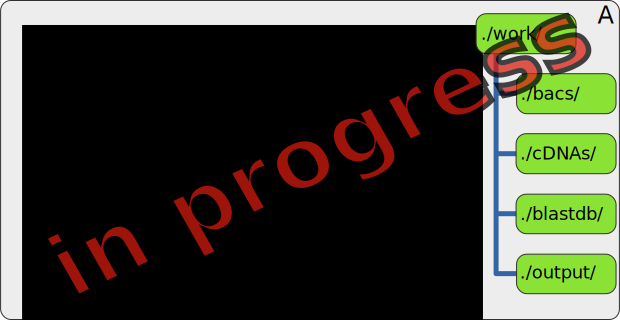
\includegraphics[width=0.9\textwidth]{image1_session.pdf}

\subsection{Image 2}
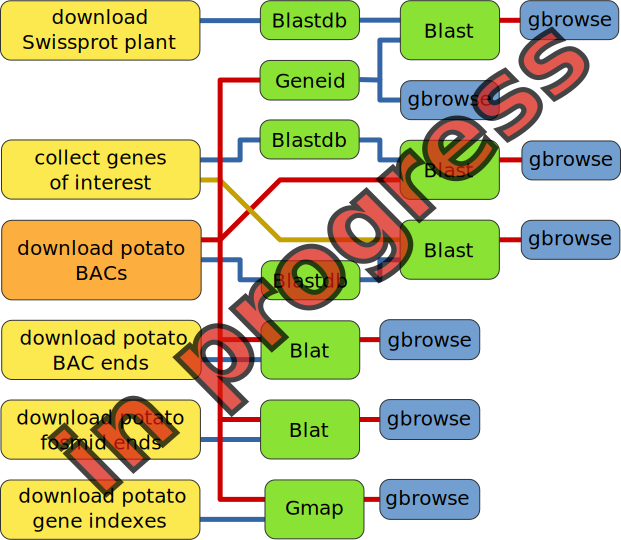
\includegraphics[width=0.9\textwidth]{image2_pipeline.pdf}


\section{Captions}

\begin{description}

\item[Figure 1], A short session on how to run Moa. The session shows
  how to use Blast to map a set of cDNA sequences against a set of
  BACs. \textit{(.. details follow..)}
\item[Figure 2], A representation of (a part of) the current potato
genome annotation pipeline. \textit{(.. details follow..)}

\end{description}

\bibliographystyle{abbrvnat}
\bibliography{poster}
\end{document}

% LocalWords:  internet Ensembl bioinformaticians Makefile workflow workflows
% LocalWords:  bioinformatics Makefiles Bowtie BAC PGSC GMap Moa posterplain
% LocalWords:  bioinformaticist
